\title[HF magnetics II]{High-frequency magnetics II: windings, planar and integrated magnetics}
\section{HF magnetics II}

\begin{frame}[plain]
	\titlepage
\end{frame}

%%%%%%%%%%%%%%%%%%%%%%%%%%%%%%%%%%%%%%%%%%%%%%%%%%%%%%%%%%%%%
%% Overview %%
%%%%%%%%%%%%%%%%%%%%%%%%%%%%%%%%%%%%%%%%%%%%%%%%%%%%%%%%%%%%%
\subsection{Winding loss at MHz}

\begin{frame}
	\frametitle{Overview}
	L6 chose the core material and the flux density. The windings decide the rest: the skin depth in copper is 47\,$\mu$m at 2\,MHz and only 18\,$\mu$m at 13.56\,MHz.
	\begin{itemize}
		\item Skin and proximity effect: Dowell's model and the optimum layer thickness
		\item Non-sinusoidal currents, litz wire and PCB windings
		\item Planar transformers: interleaving, leakage inductance, matrix and fractional-turn transformers
		\item Winding capacitance, self-resonance and common-mode paths; using the parasitics
		\item Air-core and integrated magnetics; from formula to field solver
	\end{itemize}
	After this lecture you can design the winding of a MHz inductor or planar transformer and predict its AC resistance, leakage inductance and capacitance.
\end{frame}

%%%%%%%%%%%%%%%%%%%%%%%%%%%%%%%%%%%%%%%%%%%%%%%%%%%%%%%%%%%%%
%% Skin and proximity %%
%%%%%%%%%%%%%%%%%%%%%%%%%%%%%%%%%%%%%%%%%%%%%%%%%%%%%%%%%%%%%
\begin{frame}
	\frametitle{Skin and proximity effect}
	\begin{columns}[T]
		\begin{column}{0.45\textwidth}
			\begin{figure}
				\centering
				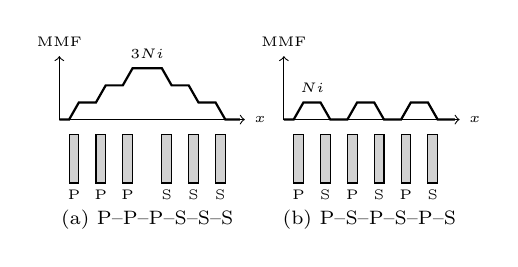
\begin{tikzpicture}[scale=0.62]
					% (a) not interleaved: P P P S S S
					\foreach \x/\l in {0.2/P,0.75/P,1.3/P,2.1/S,2.65/S,3.2/S}{
							\fill[gray!35] (\x,0) rectangle (\x+0.2,1.0);
							\draw (\x,0) rectangle (\x+0.2,1.0);
							\node[font=\tiny] at (\x+0.1,-0.25) {\l};
						}
					\draw[->] (0,1.3) -- (3.8,1.3) node[right, font=\tiny]{$x$};
					\draw[->] (0,1.3) -- (0,2.6) node[above, font=\tiny]{MMF};
					\draw[thick] (0,1.3) -- (0.2,1.3) -- (0.4,1.65) -- (0.75,1.65) -- (0.95,2.0) -- (1.3,2.0) -- (1.5,2.35) -- (2.1,2.35) -- (2.3,2.0) -- (2.65,2.0) -- (2.85,1.65) -- (3.2,1.65) -- (3.4,1.3) -- (3.7,1.3);
					\node[font=\tiny, anchor=south] at (1.8,2.35) {$3Ni$};
					\node[font=\scriptsize] at (1.8,-0.75) {(a) P--P--P--S--S--S};
					% (b) interleaved: P S P S P S
					\begin{scope}[xshift=4.6cm]
						\foreach \x/\l in {0.2/P,0.75/S,1.3/P,1.85/S,2.4/P,2.95/S}{
								\fill[gray!35] (\x,0) rectangle (\x+0.2,1.0);
								\draw (\x,0) rectangle (\x+0.2,1.0);
								\node[font=\tiny] at (\x+0.1,-0.25) {\l};
							}
						\draw[->] (0,1.3) -- (3.6,1.3) node[right, font=\tiny]{$x$};
						\draw[->] (0,1.3) -- (0,2.6) node[above, font=\tiny]{MMF};
						\draw[thick] (0,1.3) -- (0.2,1.3) -- (0.4,1.65) -- (0.75,1.65) -- (0.95,1.3) -- (1.3,1.3) -- (1.5,1.65) -- (1.85,1.65) -- (2.05,1.3) -- (2.4,1.3) -- (2.6,1.65) -- (2.95,1.65) -- (3.15,1.3) -- (3.5,1.3);
						\node[font=\tiny, anchor=south] at (0.58,1.65) {$Ni$};
						\node[font=\scriptsize] at (1.75,-0.75) {(b) P--S--P--S--P--S};
					\end{scope}
				\end{tikzpicture}
				\caption{MMF across the window: three primary (P) and three secondary (S) layers, (a) not interleaved, (b) interleaved}
			\end{figure}
		\end{column}
		\begin{column}{0.52\textwidth}
			\small
			\begin{itemize}
				\item Skin effect: the current crowds within $\delta=\sqrt{\rho/(\pi f\mu_0)}$ of the conductor surface.
				\item Proximity effect: the field of the other layers induces eddy currents. In a stack of layers the MMF grows layer by layer, and the loss of layer $m$ grows with $m^2$.
				\item In foil and PCB layers that fill the window height, the field runs parallel to the layers: a one-dimensional model works well (Dowell, 1966).
				\item Interleaving resets the MMF after each layer pair: every layer sees the field of one layer only.
			\end{itemize}
		\end{column}
	\end{columns}
	\blfootnote{Sources: Dowell, Proc.\ IEE, vol.\ 113, no.\ 8, 1966; Erickson and Maksimovi\'c, 3rd ed., 2020, Sec.\ 10.4.}
\end{frame}

%%%%%%%%%%%%%%%%%%%%%%%%%%%%%%%%%%%%%%%%%%%%%%%%%%%%%%%%%%%%%
%% Dowell %%
%%%%%%%%%%%%%%%%%%%%%%%%%%%%%%%%%%%%%%%%%%%%%%%%%%%%%%%%%%%%%
\begin{frame}
	\frametitle{Dowell's model}
	\begin{columns}[T]
		\begin{column}{0.46\textwidth}
			\begin{figure}
				\centering
				\begin{tikzpicture}
					\begin{loglogaxis}[
							width=\linewidth, height=4.6cm,
							xmin=0.1, xmax=10, ymin=0.8, ymax=200,
							xtick={0.1,1,10}, xticklabels={0.1,1,10},
							ytick={1,10,100}, yticklabels={1,10,100},
							xlabel={$\varphi=h/\delta$}, ylabel={$F_\mathrm{R}=R_\mathrm{ac}/R_\mathrm{dc}$},
							grid=major, grid style={gray!20},
							tick label style={font=\scriptsize}, label style={font=\footnotesize},
							legend style={font=\tiny}, legend pos=north west, legend cell align=left,
						]
						\addplot[black, thick] table[x=phi, y=FR6] {fig/lec07/dowell.dat};
						\addlegendentry{$M=6$}
						\addplot[black, thick, dashed] table[x=phi, y=FR4] {fig/lec07/dowell.dat};
						\addlegendentry{$M=4$}
						\addplot[gray, thick] table[x=phi, y=FR2] {fig/lec07/dowell.dat};
						\addlegendentry{$M=2$}
						\addplot[gray, thick, dashed] table[x=phi, y=FR1] {fig/lec07/dowell.dat};
						\addlegendentry{$M=1$}
					\end{loglogaxis}
				\end{tikzpicture}
				\caption{AC resistance factor of a winding with $M$ layers (sinusoidal current)}
			\end{figure}
		\end{column}
		\begin{column}{0.51\textwidth}
			\small
			\begin{equation*}
				F_\mathrm{R}=\varphi\left[G_1(\varphi)+\frac{2}{3}\left(M^2-1\right)\left(G_1(\varphi)-2G_2(\varphi)\right)\right]
			\end{equation*}
			\begin{align*}
				G_1 & =\frac{\sinh2\varphi+\sin2\varphi}{\cosh2\varphi-\cos2\varphi}                         \\
				G_2 & =\frac{\sinh\varphi\cos\varphi+\cosh\varphi\sin\varphi}{\cosh2\varphi-\cos2\varphi}
			\end{align*}
			\begin{itemize}
				\item $\varphi=h/\delta$ (foil); round wire: $\varphi=\sqrt{\eta}\,\frac{\sqrt{\pi}}{2}\frac{d}{\delta}$, porosity $\eta$.
				\item $M$: layers from zero MMF to its peak.
				\item $\varphi\gg1$: $F_\mathrm{R}\approx\varphi\,(2M^2+1)/3$.
			\end{itemize}
		\end{column}
	\end{columns}
	\blfootnote{Sources: Dowell, 1966; Erickson and Maksimovi\'c, 3rd ed., 2020, Eq.\ (10.74) and (10.87).}
\end{frame}

%%%%%%%%%%%%%%%%%%%%%%%%%%%%%%%%%%%%%%%%%%%%%%%%%%%%%%%%%%%%%
%% Optimum layer thickness %%
%%%%%%%%%%%%%%%%%%%%%%%%%%%%%%%%%%%%%%%%%%%%%%%%%%%%%%%%%%%%%
\begin{frame}
	\frametitle{Optimum layer thickness}
	\begin{columns}[T]
		\begin{column}{0.46\textwidth}
			\begin{figure}
				\centering
				\begin{tikzpicture}
					\begin{loglogaxis}[
							width=\linewidth, height=4.6cm,
							xmin=0.1, xmax=10, ymin=0.8, ymax=40,
							xtick={0.1,1,10}, xticklabels={0.1,1,10},
							ytick={1,10}, yticklabels={1,10},
							xlabel={$\varphi=h/\delta$}, ylabel={$R_\mathrm{ac}/R_\mathrm{dc}(\varphi=1)$},
							grid=major, grid style={gray!20},
							tick label style={font=\scriptsize}, label style={font=\footnotesize},
							legend style={font=\tiny}, legend pos=south west, legend cell align=left,
						]
						\addplot[black, thick] table[x=phi, y=R6] {fig/lec07/dowell.dat};
						\addlegendentry{$M=6$}
						\addplot[black, thick, dashed] table[x=phi, y=R4] {fig/lec07/dowell.dat};
						\addlegendentry{$M=4$}
						\addplot[gray, thick] table[x=phi, y=R2] {fig/lec07/dowell.dat};
						\addlegendentry{$M=2$}
						\addplot[gray, thick, dashed] table[x=phi, y=R1] {fig/lec07/dowell.dat};
						\addlegendentry{$M=1$}
					\end{loglogaxis}
				\end{tikzpicture}
				\caption{Winding resistance relative to the DC resistance of a layer with $h=\delta$}
			\end{figure}
		\end{column}
		\begin{column}{0.51\textwidth}
			\small
			Thin layers have a high DC resistance, thick layers a high proximity loss. With $F_\mathrm{R}\approx1+\frac{5M^2-1}{45}\varphi^4$ and $R\propto F_\mathrm{R}/\varphi$:
			\begin{equation*}
				\varphi_\mathrm{opt}\approx\left(\frac{15}{5M^2-1}\right)^{1/4},\qquad F_\mathrm{R}(\varphi_\mathrm{opt})\approx\frac{4}{3}
			\end{equation*}
			\begin{itemize}
				\item The more layers, the thinner each must be: $M=4$: $\varphi_\mathrm{opt}=0.66$; $M=10$: 0.42.
				\item One layer, or full interleaving: optimum at $\varphi=\pi/2$, nearly flat above $\varphi=1$.
				\item Thicker copper can raise the loss: at 2\,MHz, $M=4$ and 100\,$^\circ$C, 70\,$\mu$m copper loses 2.1 times as much as 35\,$\mu$m.
			\end{itemize}
		\end{column}
	\end{columns}
	\blfootnote{Sources: Erickson and Maksimovi\'c, 2020, Sec.\ 10.4.5--10.4.6; Hurley and W\"olfle, 2013, Sec.\ 6.3.}
\end{frame}

%%%%%%%%%%%%%%%%%%%%%%%%%%%%%%%%%%%%%%%%%%%%%%%%%%%%%%%%%%%%%
%% Task: foil thickness %%
%%%%%%%%%%%%%%%%%%%%%%%%%%%%%%%%%%%%%%%%%%%%%%%%%%%%%%%%%%%%%
% Two pages: task (page 1) and task with solution (page 2).
\begin{frame}<handout:1-2>
	\frametitle{Copper thickness at 2\,MHz}
	\begin{block}{Task (4 minutes)}
		A planar winding at 2\,MHz has $M=4$ layers in series. Copper at 100\,$^\circ$C: $\rho=2.26\cdot10^{-8}\,\Omega$m.
		\begin{enumerate}
			\item Calculate the skin depth and the optimum layer thickness.
			\item Compare 1-oz (35\,$\mu$m) and 2-oz (70\,$\mu$m) copper.
			\item Which thickness would you use at 13.56\,MHz?
		\end{enumerate}
	\end{block}
	\onslide<2-|handout:2>{
		\begin{enumerate}
			\item $\delta=\sqrt{\rho/(\pi f\mu_0)}=53.5\,\mu$m; $\varphi_\mathrm{opt}=(15/79)^{1/4}=0.66$: $h_\mathrm{opt}=35\,\mu$m.
			\item 35\,$\mu$m: $\varphi=0.65$, $F_\mathrm{R}=1.32$, optimal. 70\,$\mu$m: $\varphi=1.31$, $F_\mathrm{R}=5.6$: half the DC resistance, but 2.1 times the AC loss.
			\item $\delta=20.5\,\mu$m: four layers would need 14\,$\mu$m. Better one layer (or full interleaving): $\varphi=\pi/2$ gives 32\,$\mu$m, again 1-oz copper.
		\end{enumerate}
	}
\end{frame}

%%%%%%%%%%%%%%%%%%%%%%%%%%%%%%%%%%%%%%%%%%%%%%%%%%%%%%%%%%%%%
%% Non-sinusoidal currents %%
%%%%%%%%%%%%%%%%%%%%%%%%%%%%%%%%%%%%%%%%%%%%%%%%%%%%%%%%%%%%%
\begin{frame}
	\frametitle{Non-sinusoidal currents}
	\begin{columns}[T]
		\begin{column}{0.5\textwidth}
			\small
			Each harmonic sees its own skin depth $\delta_n=\delta_1/\sqrt{n}$:
			\begin{equation*}
				P=R_\mathrm{dc}\left[I_\mathrm{dc}^2+\sum_{n=1}^{\infty}I_n^2\,F_\mathrm{R}\!\left(\varphi_1\sqrt{n}\right)\right]
			\end{equation*}
			with rms values $I_n$ of the harmonics.
			\begin{itemize}
				\item Triangular ripple (buck, TCM): $I_n\propto1/n^2$, little extra loss.
				\item Square-wave-like currents (transformer of a hard-switched bridge): $I_n\propto1/n$, large extra loss.
				\item The optimum thickness depends on the waveform: compute it for the harmonic content.
			\end{itemize}
		\end{column}
		\begin{column}{0.47\textwidth}
			\begin{table}
				\centering
				\footnotesize
				\begin{tabular}{|l|c|c|}
					\hline
					\textbf{Current}      & $\varphi_1=0.5$ & $\varphi_1=0.66$ \\
					\hline
					sine                  & 1.11            & 1.33             \\
					triangle              & 1.13            & 1.38             \\
					square (ideal edges)  & 2.56            & 3.77             \\
					\hline
				\end{tabular}
				\caption{Effective $F_\mathrm{R}$ for $M=4$; $\varphi_1$: thickness relative to $\delta$ at the fundamental}
			\end{table}
			\small
			A layer that is optimal for a sine has almost three times the loss with a square-wave current of the same rms value.
		\end{column}
	\end{columns}
	\blfootnote{Sources: Erickson and Maksimovi\'c, 2020, Sec.\ 10.4.7; Hurley and W\"olfle, 2013, Sec.\ 6.2--6.3.}
\end{frame}

%%%%%%%%%%%%%%%%%%%%%%%%%%%%%%%%%%%%%%%%%%%%%%%%%%%%%%%%%%%%%
%% Litz wire %%
%%%%%%%%%%%%%%%%%%%%%%%%%%%%%%%%%%%%%%%%%%%%%%%%%%%%%%%%%%%%%
\begin{frame}
	\frametitle{Litz wire at MHz}
	\begin{columns}[T]
		\begin{column}{0.52\textwidth}
			\small
			\begin{itemize}
				\item Insulated strands, twisted so that each strand takes every position: the strand diameter sets skin and proximity loss.
				\item Strands must be much thinner than $\delta$. Litz becomes expensive below 50\,$\mu$m; strands below about 30\,$\mu$m are hardly available.
				\item With fixed strand diameter $R_\mathrm{ac}\propto f$: the gain of a higher frequency is lost ($\hat{B}f^{1/2}$, L6).
				\item The number of strands has an optimum: thinner strands cut the eddy-current loss, more insulation raises the DC resistance.
			\end{itemize}
		\end{column}
		\begin{column}{0.45\textwidth}
			\begin{table}
				\centering
				\footnotesize
				\begin{tabular}{|l|c|}
					\hline
					\textbf{Frequency} & $\delta$ (Cu, 20\,$^\circ$C) \\
					\hline
					100\,kHz           & 209\,$\mu$m                 \\
					1\,MHz             & 66\,$\mu$m                  \\
					6.78\,MHz          & 25\,$\mu$m                  \\
					13.56\,MHz         & 18\,$\mu$m                  \\
					\hline
				\end{tabular}
				\caption{Skin depth in copper}
			\end{table}
			\small
			Above a few MHz: single-layer solid or foil windings, PCB windings and field-balanced structures.
		\end{column}
	\end{columns}
	\blfootnote{Sources: Sullivan, IEEE TPEL, 1999; Hanson et al., IEEE TPEL, 2016; Perreault, APEC 2024 plenary.}
\end{frame}

%%%%%%%%%%%%%%%%%%%%%%%%%%%%%%%%%%%%%%%%%%%%%%%%%%%%%%%%%%%%%
%% PCB windings %%
%%%%%%%%%%%%%%%%%%%%%%%%%%%%%%%%%%%%%%%%%%%%%%%%%%%%%%%%%%%%%
\begin{frame}
	\frametitle{PCB windings}
	\begin{itemize}
		\item Copper weight: 1\,oz/ft$^2$ $\approx$ 35\,$\mu$m, 2\,oz $\approx$ 70\,$\mu$m. At 2--3\,MHz, 35\,$\mu$m is close to the optimum for two to four layers.
		\item Layers in parallel do not share the current equally: leakage fields and eddy currents drive circulating currents between them. Give each parallel layer the same field, i.e.\ the same neighbours from the other winding.
		\item Vias and terminations add AC resistance. Keep them out of the high-field region and keep the connection loops small (L3).
		\item The copper fill factor is low (insulation, prepreg, clearance): PCB windings suit few turns and high frequency.
		\item The board also spreads the heat of windings and core.
	\end{itemize}
	\begin{block}{Key message}
		A PCB winding is designed layer by layer: thickness, order and connection of the layers decide its loss.
	\end{block}
	\blfootnote{Sources: Ouyang, PhD thesis, DTU, 2011; Ranjram and Perreault, IEEE TPEL, vol.\ 37, no.\ 2, 2022.}
\end{frame}

%%%%%%%%%%%%%%%%%%%%%%%%%%%%%%%%%%%%%%%%%%%%%%%%%%%%%%%%%%%%%
%% Planar transformers %%
%%%%%%%%%%%%%%%%%%%%%%%%%%%%%%%%%%%%%%%%%%%%%%%%%%%%%%%%%%%%%
\subsection{Planar and integrated magnetics}

\begin{frame}
	\frametitle{Planar transformers}
	\begin{columns}[T]
		\begin{column}{0.45\textwidth}
			\begin{figure}
				\centering
				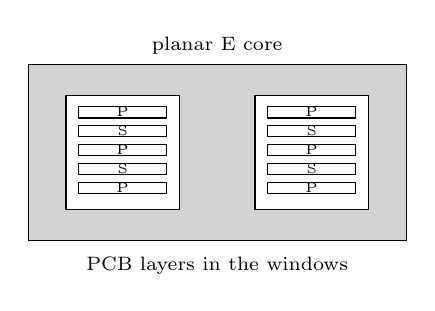
\begin{tikzpicture}[scale=0.8]
					% E core cross-section with a PCB stack in both windows
					\fill[gray!35] (0,0) rectangle (6,0.5);
					\fill[gray!35] (0,2.3) rectangle (6,2.8);
					\fill[gray!35] (0,0.5) rectangle (0.6,2.3);
					\fill[gray!35] (2.4,0.5) rectangle (3.6,2.3);
					\fill[gray!35] (5.4,0.5) rectangle (6,2.3);
					\draw (0,0) rectangle (6,2.8);
					\draw (0.6,0.5) rectangle (2.4,2.3);
					\draw (3.6,0.5) rectangle (5.4,2.3);
					\foreach \y/\l in {0.75/P,1.05/S,1.35/P,1.65/S,1.95/P}{
							\draw[fill=white] (0.8,\y) rectangle (2.2,\y+0.18);
							\draw[fill=white] (3.8,\y) rectangle (5.2,\y+0.18);
							\node[font=\tiny] at (1.5,\y+0.09) {\l};
							\node[font=\tiny] at (4.5,\y+0.09) {\l};
						}
					\node[font=\scriptsize] at (3,3.1) {planar E core};
					\node[font=\scriptsize, anchor=north] at (3,-0.1) {PCB layers in the windows};
				\end{tikzpicture}
				\caption{Cross-section of a planar transformer with interleaved PCB layers}
			\end{figure}
		\end{column}
		\begin{column}{0.52\textwidth}
			\small
			\textbf{Strengths}
			\begin{itemize}
				\item Low profile, large cooling surface, windings made with the PCB: repeatable resistance, leakage and capacitance.
				\item Rectifiers and capacitors sit directly at the winding terminals (B2, B3).
			\end{itemize}
			\textbf{Weaknesses}
			\begin{itemize}
				\item Low copper fill factor; high inter-winding capacitance when interleaved; termination loss at high current.
				\item Planar is not low-leakage by itself: interleaving gives the low leakage.
			\end{itemize}
		\end{column}
	\end{columns}
	\blfootnote{Sources: Ouyang, PhD thesis, DTU, 2011; Ranjram and Perreault, 2022.}
\end{frame}

%%%%%%%%%%%%%%%%%%%%%%%%%%%%%%%%%%%%%%%%%%%%%%%%%%%%%%%%%%%%%
%% Poll: interleaving %%
%%%%%%%%%%%%%%%%%%%%%%%%%%%%%%%%%%%%%%%%%%%%%%%%%%%%%%%%%%%%%
% Two pages: question (page 1) and answer (page 2).
\begin{frame}<handout:1-2>
	\frametitle{What interleaving does}
	A planar transformer is changed from P--P--S--S to P--S--P--S. Vote, then discuss with your neighbour (2 minutes). Interleaving \dots
	\begin{enumerate}[(a)]
		\item reduces proximity loss and leakage, but increases the inter-winding capacitance
		\item reduces the inter-winding capacitance, but increases the leakage
		\item reduces the core loss
		\item reduces the DC resistance
	\end{enumerate}
	\onslide<2-|handout:2>{
		\begin{block}{Answer: (a)}
			The MMF peak halves, so each layer works with $m=1$ and the field energy in the window (the leakage) drops. Every P--S interface, however, adds a capacitance $C=\varepsilon_0\varepsilon_\mathrm{r}A/d$: for an overlap of 40\,mm $\times$ 8\,mm and 0.2\,mm FR4 ($\varepsilon_\mathrm{r}=4.4$) this is 62\,pF. A switching edge of 50\,V/ns drives 3.1\,A through it, into the secondary ground. Core loss and DC resistance do not change.
		\end{block}
	}
\end{frame}

%%%%%%%%%%%%%%%%%%%%%%%%%%%%%%%%%%%%%%%%%%%%%%%%%%%%%%%%%%%%%
%% Leakage inductance %%
%%%%%%%%%%%%%%%%%%%%%%%%%%%%%%%%%%%%%%%%%%%%%%%%%%%%%%%%%%%%%
\begin{frame}
	\frametitle{Leakage inductance}
	\begin{columns}[T]
		\begin{column}{0.44\textwidth}
			\begin{figure}
				\centering
				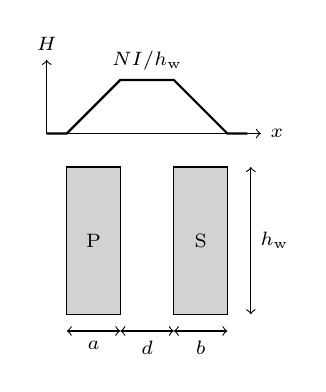
\begin{tikzpicture}[scale=0.85]
					\fill[gray!35] (0.5,0) rectangle (1.3,2.2);
					\fill[gray!35] (2.1,0) rectangle (2.9,2.2);
					\draw (0.5,0) rectangle (1.3,2.2);
					\draw (2.1,0) rectangle (2.9,2.2);
					\node[font=\scriptsize] at (0.9,1.1) {P};
					\node[font=\scriptsize] at (2.5,1.1) {S};
					\draw[<->] (0.5,-0.25) -- (1.3,-0.25) node[midway, below, font=\scriptsize]{$a$};
					\draw[<->] (1.3,-0.25) -- (2.1,-0.25) node[midway, below, font=\scriptsize]{$d$};
					\draw[<->] (2.1,-0.25) -- (2.9,-0.25) node[midway, below, font=\scriptsize]{$b$};
					\draw[<->] (3.25,0) -- (3.25,2.2) node[midway, right, font=\scriptsize]{$h_\mathrm{w}$};
					% H profile
					\draw[->] (0.2,2.7) -- (3.4,2.7) node[right, font=\scriptsize]{$x$};
					\draw[->] (0.2,2.7) -- (0.2,3.8) node[above, font=\scriptsize]{$H$};
					\draw[thick] (0.2,2.7) -- (0.5,2.7) -- (1.3,3.5) -- (2.1,3.5) -- (2.9,2.7) -- (3.2,2.7);
					\node[font=\scriptsize, anchor=south] at (1.7,3.5) {$NI/h_\mathrm{w}$};
				\end{tikzpicture}
				\caption{Window cross-section and field between primary and secondary}
			\end{figure}
		\end{column}
		\begin{column}{0.53\textwidth}
			\small
			Energy in the window, $W=\frac{\mu_0}{2}\int H^2\,\mathrm{d}V$, with the mean turn length MLT:
			\begin{equation*}
				L_\mathrm{lk}=\frac{\mu_0N^2\,\mathrm{MLT}}{h_\mathrm{w}}\left(d+\frac{a+b}{3}\right)
			\end{equation*}
			\begin{itemize}
				\item Low leakage: few turns, thin windings, small gap, wide window, interleaving.
				\item Example: $N=4$, MLT = 40\,mm, $h_\mathrm{w}=8$\,mm, $a=b=d=0.2$\,mm: $L_\mathrm{lk}=34$\,nH.
				\item Eddy currents push the field out of thick conductors: for $h=2\delta$ the leakage is 25--30\,\% lower. Use this value when the leakage is the resonant inductor.
			\end{itemize}
		\end{column}
	\end{columns}
	\blfootnote{Sources: Hurley and W\"olfle, 2013, Sec.\ 6.5; Dowell, 1966.}
\end{frame}

%%%%%%%%%%%%%%%%%%%%%%%%%%%%%%%%%%%%%%%%%%%%%%%%%%%%%%%%%%%%%
%% Matrix and fractional-turn transformers %%
%%%%%%%%%%%%%%%%%%%%%%%%%%%%%%%%%%%%%%%%%%%%%%%%%%%%%%%%%%%%%
\begin{frame}
	\frametitle{Matrix and fractional-turn transformers}
	\begin{columns}[T]
		\begin{column}{0.49\textwidth}
			\small
			\textbf{Matrix transformer}
			\begin{itemize}
				\item Several small transformers, primaries in series, secondaries in parallel, each with its own synchronous rectifier.
				\item Shared core legs cancel part of the flux.
				\item Huang, Ji, Lee: 1\,kW, 390\,V to 12\,V, 1\,MHz, 95.4\,\% peak efficiency, about 830\,W/in$^3$ power stage.
			\end{itemize}
		\end{column}
		\begin{column}{0.48\textwidth}
			\small
			\textbf{Split-phase fractional-turn transformer}
			\begin{itemize}
				\item The secondary behaves as a fraction of a turn; several phases share the current.
				\item Ranjram and Perreault: 380\,V to 12\,V, 1\,kW, 1\,MHz, 97.7\,\% peak and 97.1\,\% full-load efficiency, transformer and rectifiers in 14.2\,cm$^3$, 12--36\,\% smaller than the best designs of the same power.
			\end{itemize}
		\end{column}
	\end{columns}
	\begin{block}{Key message}
		At high step-down ratio and high current the secondary and its terminations dominate. Splitting the transformer and paralleling the secondaries reduces the copper loss.
	\end{block}
	\blfootnote{Sources: Huang, Ji, Lee, IEEE TPEL, 2014; Ranjram and Perreault, IEEE TPEL, 2022.}
\end{frame}

%%%%%%%%%%%%%%%%%%%%%%%%%%%%%%%%%%%%%%%%%%%%%%%%%%%%%%%%%%%%%
%% Integrated magnetics %%
%%%%%%%%%%%%%%%%%%%%%%%%%%%%%%%%%%%%%%%%%%%%%%%%%%%%%%%%%%%%%
\begin{frame}
	\frametitle{Integrated magnetics}
	\begin{itemize}
		\item Coupled inductors in multiphase buck converters: inversely coupled windings on one core lower the ripple of each phase for the same transient response.
		\item Transformer with integrated resonant inductor: the leakage, or a magnetic shunt, provides $L_\mathrm{r}$ of an LLC (B2) or the series inductance of a DAB (B3).
		\item Matrix transformers share core legs and cancel flux.
		\item Fewer components and less core volume, but coupling and leakage must be designed and measured: they now set the converter behaviour.
	\end{itemize}
	\blfootnote{Sources: P.-L. Wong, PhD thesis, Virginia Tech, 2001; Ouyang, PhD thesis, DTU, 2011; Huang, Ji, Lee, 2014.}
\end{frame}

%%%%%%%%%%%%%%%%%%%%%%%%%%%%%%%%%%%%%%%%%%%%%%%%%%%%%%%%%%%%%
%% Design sprint %%
%%%%%%%%%%%%%%%%%%%%%%%%%%%%%%%%%%%%%%%%%%%%%%%%%%%%%%%%%%%%%
% Two pages: task (page 1) and task with solution (page 2).
\begin{frame}<handout:1-2>
	\frametitle{Layer stack of a 4:1 transformer}
	\begin{block}{Task (6 minutes, in teams)}
		Planar transformer for B2: 48\,V to 12\,V, 250\,W, 1\,MHz, 4:1. Eight PCB layers with 35\,$\mu$m copper; four primary turns, one secondary turn.
		\begin{enumerate}
			\item Allocate the turns to the layers and choose the order of the layers.
			\item Which layers do you connect in parallel, and why?
			\item How do leakage and inter-winding capacitance compare with the stack PPPP--SSSS?
		\end{enumerate}
	\end{block}
	\onslide<2-|handout:2>{
		\small
		One good solution:
		\begin{enumerate}
			\item P--S--P--S--S--P--S--P. Primary: two turns per layer, two layers in series, two such halves in parallel. Secondary: one turn per layer, four layers in parallel.
			\item Every layer carries the same ampere-turns next to a layer of the other winding: the MMF stays below $N_\mathrm{p}I_\mathrm{p}/4$ and parallel layers share the current.
			\item 1-D estimate (0.1\,mm between layers): about 12 times less leakage than PPPP--SSSS, but six P--S interfaces instead of one: about six times the capacitance.
		\end{enumerate}
	}
\end{frame}

%%%%%%%%%%%%%%%%%%%%%%%%%%%%%%%%%%%%%%%%%%%%%%%%%%%%%%%%%%%%%
%% Winding capacitance %%
%%%%%%%%%%%%%%%%%%%%%%%%%%%%%%%%%%%%%%%%%%%%%%%%%%%%%%%%%%%%%
\subsection{Parasitic capacitance}

\begin{frame}
	\frametitle{Winding capacitance}
	\begin{columns}[T]
		\begin{column}{0.4\textwidth}
			\begin{figure}
				\centering
				\begin{circuitikz}[scale=0.9, transform shape]
					\draw (0,0) to[L, l=$L$] (2,0) to[R, l=$R_\mathrm{ac}$] (4,0);
					\draw (0,0) -- (0,-1.3) to[C, l_=$C_\mathrm{w}$] (4,-1.3) -- (4,0);
					\draw (0,0) -- (-0.4,0) node[circ]{};
					\draw (4,0) -- (4.4,0) node[circ]{};
				\end{circuitikz}
				\caption{Lumped model of a winding}
			\end{figure}
			\small
			\begin{equation*}
				f_\mathrm{SRF}=\frac{1}{2\pi\sqrt{LC_\mathrm{w}}}
			\end{equation*}
			Above $f_\mathrm{SRF}$ the winding behaves as a capacitor.
		\end{column}
		\begin{column}{0.57\textwidth}
			\small
			\begin{itemize}
				\item Turn-to-turn and layer-to-layer capacitances store electric energy. Lumped into $C_\mathrm{w}$, they set the self-resonance.
				\item Energy method: adjacent layers with capacitance $C_0$, voltage linear along the winding. Layers wound back and forth:
				      \begin{equation*}
					      C_\mathrm{w}=\frac{4}{3}C_0\frac{n-1}{n^2}
				      \end{equation*}
				      For $n=2$: $C_0/3$. If every layer starts at the same side (return wire needed): $C_0(n-1)/n^2$, for $n=2$: $C_0/4$.
				\item Few layers, larger spacing between layers and sectioned windings lower $C_\mathrm{w}$; in multilayer windings the layer-to-layer capacitance dominates.
			\end{itemize}
		\end{column}
	\end{columns}
	\blfootnote{Source: Massarini and Kazimierczuk, IEEE TPEL, vol.\ 12, no.\ 4, 1997.}
\end{frame}

%%%%%%%%%%%%%%%%%%%%%%%%%%%%%%%%%%%%%%%%%%%%%%%%%%%%%%%%%%%%%
%% Task: self-resonance %%
%%%%%%%%%%%%%%%%%%%%%%%%%%%%%%%%%%%%%%%%%%%%%%%%%%%%%%%%%%%%%
% Two pages: task (page 1) and task with solution (page 2).
\begin{frame}<handout:1-2>
	\frametitle{Self-resonance}
	\begin{block}{Task (3 minutes)}
		\begin{enumerate}
			\item A 10\,$\mu$H inductor of an EMI filter has 5\,pF winding capacitance. Where is its self-resonance?
			\item Up to which harmonic of a 2\,MHz converter does it act as an inductor?
			\item Which $C_\mathrm{w}$ may a 1\,$\mu$H inductor have, if it must stay inductive up to 100\,MHz?
		\end{enumerate}
	\end{block}
	\onslide<2-|handout:2>{
		\begin{enumerate}
			\item $f_\mathrm{SRF}=1/(2\pi\sqrt{10\,\mu\mathrm{H}\cdot5\,\mathrm{pF}})=22.5$\,MHz.
			\item Up to the 11th harmonic. Above, the HF current bypasses the inductor through $C_\mathrm{w}$ and the filter loses its attenuation.
			\item $C_\mathrm{w}<1/((2\pi\cdot100\,\mathrm{MHz})^2\cdot1\,\mu\mathrm{H})=2.5$\,pF: a single-layer winding, or several sections in series.
		\end{enumerate}
	}
\end{frame}

%%%%%%%%%%%%%%%%%%%%%%%%%%%%%%%%%%%%%%%%%%%%%%%%%%%%%%%%%%%%%
%% Inter-winding capacitance %%
%%%%%%%%%%%%%%%%%%%%%%%%%%%%%%%%%%%%%%%%%%%%%%%%%%%%%%%%%%%%%
\begin{frame}
	\frametitle{Inter-winding capacitance}
	\begin{itemize}
		\item The capacitance $C_\mathrm{ps}$ between primary and secondary couples the switching edges into the secondary: $i_\mathrm{CM}=C_\mathrm{ps}\,\mathrm{d}v/\mathrm{d}t$ returns through ground and the LISN (L14).
		\item Example from the poll: 62\,pF per interface. Hard switching at 50\,V/ns: 3.1\,A; a ZVS transition at 5\,V/ns: 0.3\,A.
		\item A shield layer between primary and secondary, connected to a quiet primary node, returns this current locally. It must not form a shorted turn: thin, and open at one point.
		\item Symmetric windings and balanced edges (full bridge) let the injected currents cancel.
	\end{itemize}
	\begin{block}{Key message}
		Interleaving, shields and soft switching are designed together: low leakage and low common-mode current pull in opposite directions.
	\end{block}
	\blfootnote{Sources: Ott, \textit{Electromagnetic Compatibility Engineering}, 2009, Sec.\ 13.2.1; Ouyang, PhD thesis, DTU, 2011.}
\end{frame}

%%%%%%%%%%%%%%%%%%%%%%%%%%%%%%%%%%%%%%%%%%%%%%%%%%%%%%%%%%%%%
%% Using parasitics %%
%%%%%%%%%%%%%%%%%%%%%%%%%%%%%%%%%%%%%%%%%%%%%%%%%%%%%%%%%%%%%
\begin{frame}
	\frametitle{Using the parasitics}
	\begin{columns}[T]
		\begin{column}{0.5\textwidth}
			\small
			\begin{itemize}
				\item The leakage inductance becomes the resonant inductor of an LLC (B2) or the series inductor of a DAB (B3). A planar stack makes it repeatable.
				\item Winding capacitance and $C_\mathrm{oss}$ become part of the resonant capacitance of class E and $\Phi_2$ converters (B4, B5; L10).
				\item What cannot be absorbed must be small: a parasitic is a component that was not designed.
			\end{itemize}
		\end{column}
		\begin{column}{0.47\textwidth}
			\small
			\textbf{Inductance cancellation}
			\begin{itemize}
				\item The parasitic inductance (ESL) of a filter capacitor limits its attenuation at HF.
				\item Two coupled PCB windings in the capacitor branch create a negative mutual inductance that cancels the ESL.
				\item The filter keeps its attenuation to much higher frequency without larger components.
			\end{itemize}
		\end{column}
	\end{columns}
	\blfootnote{Source: Neugebauer and Perreault, IEEE TPEL, vol.\ 19, no.\ 3, 2004.}
\end{frame}

%%%%%%%%%%%%%%%%%%%%%%%%%%%%%%%%%%%%%%%%%%%%%%%%%%%%%%%%%%%%%
%% Air core and high Q %%
%%%%%%%%%%%%%%%%%%%%%%%%%%%%%%%%%%%%%%%%%%%%%%%%%%%%%%%%%%%%%
\subsection{Beyond ferrite cores}

\begin{frame}
	\frametitle{Air-core and high-$Q$ inductors}
	\begin{columns}[T]
		\begin{column}{0.5\textwidth}
			\small
			\textbf{Air core}
			\begin{itemize}
				\item No core loss and no saturation, linear: the choice at VHF (B5) and in RF matching.
				\item $Q$ is limited by the copper: with $R_\mathrm{ac}\propto\sqrt{f}$, $Q\propto\sqrt{f}$ up to the self-resonance.
				\item The field extends outside: keep metal and other loops away, or use toroidal PCB coils.
			\end{itemize}
		\end{column}
		\begin{column}{0.47\textwidth}
			\small
			\textbf{High-$Q$ cored inductors}
			\begin{itemize}
				\item Yang et al.\ (2019): quasi-distributed gaps and double-sided conduction, 15\,$\mu$H at 3\,MHz: $Q=720$, 980 with litz wire.
				\item Joisher et al.\ (2024): 570\,nH at 13.56\,MHz, $Q=1150$ at 80\,A peak, self-shielded, 1.6\,litre.
			\end{itemize}
		\end{column}
	\end{columns}
	\blfootnote{Sources: Yang et al., IEEE TPEL, 2019; Joisher et al., IEEE APEC 2024; Perreault, APEC 2024 plenary.}
\end{frame}

%%%%%%%%%%%%%%%%%%%%%%%%%%%%%%%%%%%%%%%%%%%%%%%%%%%%%%%%%%%%%
%% On chip and in package %%
%%%%%%%%%%%%%%%%%%%%%%%%%%%%%%%%%%%%%%%%%%%%%%%%%%%%%%%%%%%%%
\begin{frame}
	\frametitle{Magnetics in the package}
	\begin{columns}[T]
		\begin{column}{0.5\textwidth}
			\small
			\textbf{Intel FIVR (2014)}
			\begin{itemize}
				\item Multiphase buck converters at 140\,MHz, up to 16 phases each, 8 to 31 regulators per processor.
				\item Air-core inductors made from the metal layers of the package.
				\item About 90\,\% peak efficiency from 1.7\,V to 1.05\,V; 31\,A/mm$^2$.
			\end{itemize}
		\end{column}
		\begin{column}{0.47\textwidth}
			\small
			\textbf{Power supply on chip}
			\begin{itemize}
				\item Thin magnetic films (NiFe, CoZrTa, Co-Zr-O) raise the inductance per area at 10--100\,MHz.
				\item The scaling laws of L6 still hold: small inductors are limited by efficiency. Integration pays at low voltage, low power per phase and very high current density.
			\end{itemize}
		\end{column}
	\end{columns}
	\blfootnote{Sources: Burton et al., IEEE APEC 2014, pp.\ 432--439; \'O Math\'una et al., IEEE TPEL, vol.\ 27, no.\ 11, 2012.}
\end{frame}

%%%%%%%%%%%%%%%%%%%%%%%%%%%%%%%%%%%%%%%%%%%%%%%%%%%%%%%%%%%%%
%% Modelling workflow %%
%%%%%%%%%%%%%%%%%%%%%%%%%%%%%%%%%%%%%%%%%%%%%%%%%%%%%%%%%%%%%
\subsection{Design and modelling}

\begin{frame}
	\frametitle{From formula to field solver}
	\begin{table}
		\centering
		\footnotesize
		\begin{tabular}{|>{\raggedright\arraybackslash}p{2.6cm}|>{\raggedright\arraybackslash}p{4.6cm}|>{\raggedright\arraybackslash}p{5.6cm}|}
			\hline
			\textbf{Method}                         & \textbf{Gives}                                                 & \textbf{Limits}                                                                  \\
			\hline
			Dowell, 1-D energy method               & $F_\mathrm{R}$, optimum thickness, leakage, in seconds         & 1-D field: no gap fringing, no end turns, no terminations                        \\
			2-D FEM (FEMM, FEMMT)                   & current distribution, losses, inductance matrix, fringing      & axisymmetric or planar cut; FEMMT: open-source Python, litz and core loss models  \\
			3-D FEM                                 & end turns, terminations, planar stacks                          & mesh and run time; check against measurement                                     \\
			Measurement                             & $L$, $R_\mathrm{ac}(f)$, $f_\mathrm{SRF}$, leakage (L5)         & fixture and calibration; core loss by the resonant method                        \\
			\hline
		\end{tabular}
		\caption{Modelling tools for HF magnetic components}
	\end{table}
	\small
	Use the analytical model to choose the design, the field solver to check what the 1-D model ignores, and the measurement to close the loop.
	\blfootnote{Sources: FEMM (D.\,Meeker); FEMMT, Paderborn University, github.com/upb-lea/FEM\_Magnetics\_Toolbox.}
\end{frame}

%%%%%%%%%%%%%%%%%%%%%%%%%%%%%%%%%%%%%%%%%%%%%%%%%%%%%%%%%%%%%
%% Design flow %%
%%%%%%%%%%%%%%%%%%%%%%%%%%%%%%%%%%%%%%%%%%%%%%%%%%%%%%%%%%%%%
\begin{frame}
	\frametitle{Design flow for a planar transformer}
	\begin{columns}[T]
		\begin{column}{0.5\textwidth}
			\small
			\begin{enumerate}
				\item Specification: voltages, currents and waveforms, frequency, space, temperature.
				\item Core and material from the performance factor (L6).
				\item Turns from the optimum $\hat{B}$ and integer turns ratio; core loss with the iGSE.
				\item Layer stack: thickness from Dowell for the actual harmonics, interleaving, paralleling.
				\item Leakage and capacitance: do they fit the topology (resonant inductor, ZVS, common mode)?
				\item Field-solver check, prototype, measurement.
			\end{enumerate}
		\end{column}
		\begin{column}{0.47\textwidth}
			\small
			\textbf{Typical iterations}
			\begin{itemize}
				\item Too much winding loss: fewer layers, interleave, thinner copper for square-wave currents.
				\item Too much leakage: interleave; too much capacitance: fewer interfaces, shield.
				\item Termination loss at the secondary: matrix or fractional-turn structure.
			\end{itemize}
		\end{column}
	\end{columns}
\end{frame}

%%%%%%%%%%%%%%%%%%%%%%%%%%%%%%%%%%%%%%%%%%%%%%%%%%%%%%%%%%%%%
%% Windings in the briefs %%
%%%%%%%%%%%%%%%%%%%%%%%%%%%%%%%%%%%%%%%%%%%%%%%%%%%%%%%%%%%%%
\begin{frame}
	\frametitle{Windings in the briefs}
	\begin{table}
		\centering
		\footnotesize
		\begin{tabular}{|l|>{\raggedright\arraybackslash}p{3.0cm}|>{\raggedright\arraybackslash}p{9.6cm}|}
			\hline
			   & \textbf{Brief}           & \textbf{Winding question}                                                                                    \\
			\hline
			B1 & ZVS GaN buck, 1--3\,MHz  & inductor winding with DC and large triangular ripple: $F_\mathrm{R}$ of the harmonics; distance to the gap  \\
			B2 & LLC DCX, 1\,MHz          & 4:1 planar stack, about 21\,A on the secondary: interleaving, paralleling, terminations                      \\
			B3 & DAB, 0.5--1\,MHz         & leakage as series inductance: value at the operating frequency, tolerance                                    \\
			B4 & 6.78\,MHz class E        & coil and matching inductors: $Q$ and self-resonance                                                          \\
			B5 & 13.56\,MHz VHF           & air-core inductors: $Q$, self-resonance, stray field and layout                                              \\
			B6 & hybrid SC, 48\,V         & small resonant inductors: PCB or SMD, DC resistance and AC loss                                              \\
			\hline
		\end{tabular}
		\caption{Milestone M1 (25.11.): magnetics pre-design with winding concept}
	\end{table}
\end{frame}

%%%%%%%%%%%%%%%%%%%%%%%%%%%%%%%%%%%%%%%%%%%%%%%%%%%%%%%%%%%%%
%% Key messages %%
%%%%%%%%%%%%%%%%%%%%%%%%%%%%%%%%%%%%%%%%%%%%%%%%%%%%%%%%%%%%%
\begin{frame}
	\frametitle{Key messages}
	\begin{enumerate}
		\item Skin depth in copper: 66\,$\mu$m at 1\,MHz, 21\,$\mu$m at 10\,MHz. In multilayer windings the proximity effect dominates; the loss grows with $M^2$.
		\item Optimum layer thickness $\varphi_\mathrm{opt}\approx(15/(5M^2-1))^{1/4}$ with $F_\mathrm{R}\approx4/3$; thicker copper can raise the loss.
		\item Non-sinusoidal currents: sum the harmonics. Square-wave currents need thinner layers or interleaving.
		\item Interleaving lowers proximity loss and leakage and raises the inter-winding capacitance.
		\item Leakage follows from the field energy and falls at HF; winding capacitance sets the self-resonance; inter-winding capacitance is a common-mode path.
		\item Above a few MHz litz wire loses its advantage: single-layer, foil, PCB, field-balanced and air-core windings.
	\end{enumerate}
\end{frame}

%%%%%%%%%%%%%%%%%%%%%%%%%%%%%%%%%%%%%%%%%%%%%%%%%%%%%%%%%%%%%
%% Exit ticket %%
%%%%%%%%%%%%%%%%%%%%%%%%%%%%%%%%%%%%%%%%%%%%%%%%%%%%%%%%%%%%%
% Two pages: questions (page 1) and answers (page 2).
\begin{frame}<handout:1-2>
	\frametitle{Exit questions}
	\begin{varblock}[\textwidth]{Three questions, one minute each}
		\begin{enumerate}
			\item Which foil thickness minimises the loss of a two-layer winding at 1\,MHz ($\delta=66\,\mu$m)?
			\item Why does interleaving raise the common-mode current of a converter?
			\item The leakage inductance of a transformer was measured as 100\,nH at 100\,kHz. Does the LLC tank see 100\,nH at 1\,MHz?
		\end{enumerate}
	\end{varblock}
	\onslide<2-|handout:2>{
		\begin{enumerate}
			\item $\varphi_\mathrm{opt}=(15/19)^{1/4}=0.94$: $h=62\,\mu$m.
			\item More primary--secondary interfaces give more capacitance; $i=C\,\mathrm{d}v/\mathrm{d}t$.
			\item Not necessarily: if the layers are thicker than about $\delta$ at 1\,MHz, eddy currents lower the leakage. Measure at the operating frequency.
		\end{enumerate}
	}
\end{frame}

%%%%%%%%%%%%%%%%%%%%%%%%%%%%%%%%%%%%%%%%%%%%%%%%%%%%%%%%%%%%%
%% References %%
%%%%%%%%%%%%%%%%%%%%%%%%%%%%%%%%%%%%%%%%%%%%%%%%%%%%%%%%%%%%%
\begin{frame}
	\frametitle{References}
	\scriptsize
	\begin{itemize}
		\item P.\,L. Dowell, ``Effects of eddy currents in transformer windings,'' Proc.\ IEE, vol.\ 113, no.\ 8, pp.\ 1387--1394, 1966.
		\item R.\,W. Erickson, D. Maksimovi\'c, \textit{Fundamentals of Power Electronics}, 3rd ed., Springer, 2020, Ch.\ 10--12.
		\item W.\,G. Hurley, W.\,H. W\"olfle, \textit{Transformers and Inductors for Power Electronics}, Wiley, 2013, Ch.\ 6.
		\item C.\,R. Sullivan, ``Optimal choice for number of strands in a litz-wire transformer winding,'' IEEE Trans.\ Power Electron., vol.\ 14, no.\ 2, pp.\ 283--291, 1999.
		\item Z. Ouyang, \textit{Advances in Planar and Integrated Magnetics}, PhD thesis, Technical University of Denmark, 2011.
		\item D. Huang, S. Ji, F.\,C. Lee, ``LLC resonant converter with matrix transformer,'' IEEE Trans.\ Power Electron., vol.\ 29, no.\ 8, pp.\ 4339--4347, 2014.
		\item M.\,K. Ranjram, D.\,J. Perreault, ``A 380-12\,V, 1-kW, 1-MHz converter using a miniaturized split-phase, fractional-turn planar transformer,'' IEEE Trans.\ Power Electron., vol.\ 37, no.\ 2, pp.\ 1666--1681, 2022.
		\item A. Massarini, M.\,K. Kazimierczuk, ``Self-capacitance of inductors,'' IEEE Trans.\ Power Electron., vol.\ 12, no.\ 4, pp.\ 671--676, 1997.
	\end{itemize}
\end{frame}

\begin{frame}
	\frametitle{References (cont.)}
	\scriptsize
	\begin{itemize}
		\item T.\,C. Neugebauer, D.\,J. Perreault, ``Filters with inductance cancellation using printed circuit board transformers,'' IEEE Trans.\ Power Electron., vol.\ 19, no.\ 3, pp.\ 591--602, 2004.
		\item R.\,S. Yang et al., ``A low-loss inductor structure and design guidelines for high-frequency applications,'' IEEE Trans.\ Power Electron., vol.\ 34, no.\ 10, pp.\ 9993--10005, 2019.
		\item M. Joisher et al., ``High-performance high-power inductor design for high-frequency applications,'' IEEE APEC 2024.
		\item E.\,A. Burton et al., ``FIVR -- Fully integrated voltage regulators on 4th generation Intel Core SoCs,'' IEEE APEC 2014, pp.\ 432--439.
		\item C. \'O Math\'una, N. Wang, S. Kulkarni, S. Roy, ``Review of integrated magnetics for power supply on chip (PwrSoC),'' IEEE Trans.\ Power Electron., vol.\ 27, no.\ 11, pp.\ 4799--4816, 2012.
		\item P.-L. Wong, \textit{Performance Improvements of Multi-Channel Interleaving Voltage Regulator Modules with Integrated Coupling Inductors}, PhD thesis, Virginia Tech, 2001.
		\item H.\,W. Ott, \textit{Electromagnetic Compatibility Engineering}, Wiley, 2009, Ch.\ 13.
		\item FEMM (D. Meeker); FEMMT -- FEM Magnetics Toolbox, Paderborn University (open source).
	\end{itemize}
\end{frame}
